\begin{figure}
  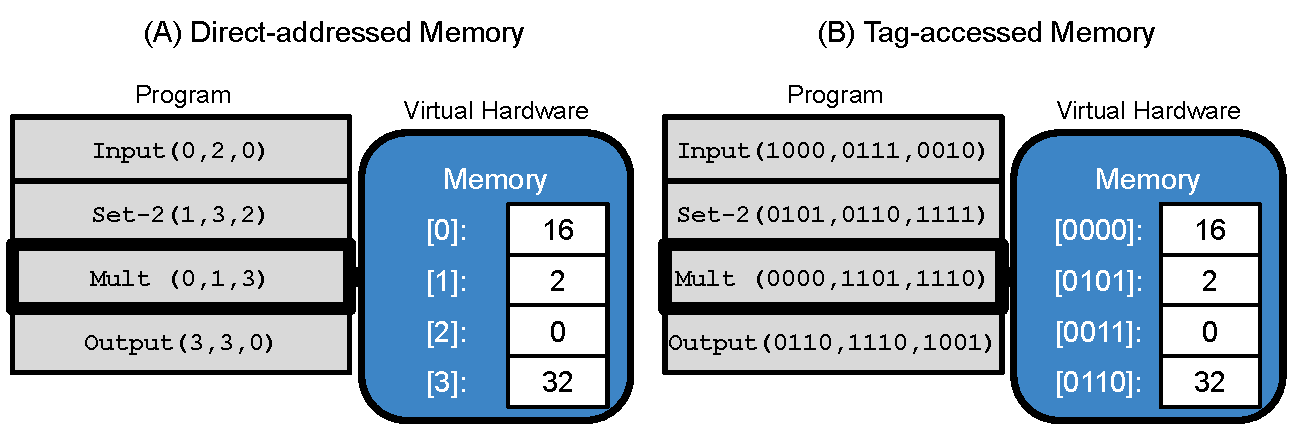
\includegraphics[width=1.0\columnwidth]{chapters/06-tag-access-memory/media/memory-access-overview.pdf}
  \caption{\small 
  \textbf{Examples of (A) direct-indexed memory and (B) tag-accessed memory. }
  The programs in (A) and (B) behave identically: both request input to the first memory register, set the second memory register to the terminal value ``2'', place the result of multiplying the contents of the first two memory registers into the fourth memory register, and output the contents of the fourth register.
  Here, we show the state of memory after the \code{Mult} instruction has been executed. 
  Note that not all instructions use all three arguments.
  }
  \label{chapter:tag-accessed-memory:fig:memory-access-overview}
\end{figure}